Wewnątrz tego rozdziału znajduje się krótki opis aplikacji służącej do przeprowadzenia analizy punktów, deskrypcja wykorzystanych narzędzi, jak również specyfikacje wewnętrzna i zewnętrzna aplikacji. W specyfikacji zewnętrznej znajdziemy opis parametrów uruchomieniowych programu, sposób formatowania danych wejściowych oraz wyjściowych oraz podgląd danych wyjściowych. Dla specyfikacji wewnętrznej przygotowano opis wymagań aplikacji, sposób kalibracji danych wejściowych. Zaprezentowano również fragmenty kodu przedstawiające obsługę silnika MongoDB dla platformy Python, metodę przygotowania danych do analizy za pomocą algorytmów I-VT oraz I-DT. Następnie przedstawiono implementację trzech algorytmów - I-VT, I-DT oraz algorytmu korzystającego z uczenia maszynowego. Ostatnie trzy sekcje prezentują metody odpowiadające za prezentację wyników, pomiar czasu oraz pomiar wykorzystania pamięci. 
\section{Krótki opis aplikacji}
\label{sec:shortdesc}
Program, który został wykorzystany do analizy punktów pomiarowych został przygotowany jako aplikacja konsolowa. Tego typu aplikacja pozwala na implementację algorytmów, jak również różnych sposobów wykonywania pomiarów, bez obciążania maszyny o zbędne GUI\footnote{z ang. Graphical User Interface - graficzny interfejs użytkownika}, który może powodować przekłamania względem analizy czasowej i pamięciowej. Aplikacja wykorzystuje bazę danych MongoDB, będącej bazą typu NoSQL. Zastosowano to rozwiązanie celem weryfikacji różnicy w łącznym czasie trwania aplikacji w stosunku do pobierania danych z pliku. W tabeli \ref{tab:nosqlschema} zeprezentowano schemat tabeli z elementami.
\begin{table}[H]
    \centering
    \begin{tabular}{|l|l|}
    \hline
    \textbf{Nazwa} & \textbf{Typ danych} \\ \hline
    \_id           & ObjectId \textit{Unique PK} \\ \hline
    Type           & String              \\ \hline
    CoordX         & Double              \\ \hline
    CoordY         & Double              \\ \hline
    TimeStamp      & String              \\ \hline
    \end{tabular}
    \caption{Schemat tabeli z elementami}
    \label{tab:nosqlschema}
\end{table}
Jak można zaobserwować na schemacie, identyfikator tabeli jest kluczem głównym, unikalnym, generowanym automatycznie przez silnik bazodanowy. Następne pola odpowiadają wartościom zaprezentowanym przy analizie danych wejściowych opisanej w sekcji \ref{ssec:importdata}.\par
W założeniu aplikacja działa w następujący sposób.
\begin{enumerate}
        \item Podając odpowiednie parametry wejściowe uruchom aplikację.
        \item Pobierz dane wejściowe z wybranego źródła.
        \item Skalibruj te dane do formatu danych odpowiadających punktom 'SS'
        \item Dla grupy punktów o typie 'R' oddzielonej punktem posiadającym parametr 'SS' uruchom wybrany algorytm
        \item Zaprezentuj wynik algorytmu na rysunku dla użytkownika
        \item Zapisz dane wyjściowe do plików
\end{enumerate}
Dokładny opis działania każdego z powyższych punktów zaprezentowano w sekcji \ref{sec:internal}.
\section{Wykorzystane narzędzia}
\label{sec:tools}
Projekt został stworzony wykorzystując język programowania \emph{Python} \cite{Python} w wersji 3.7.3. Ten język został wybrany ze względu na jego czytelność oraz modułowość. Kolejnym czynnikiem przeważającym w wyborze, była prostota w implementacji algorytmów, ze względu na wykorzystanie gotowych funkcjonalności języka Python. Rozważanymi alternatywami był język \emph{F\#} oraz język \emph{R}. Język F\# wykorzystuje platformę .NET, co na pewno ułatwiło by rozwiązanie problemu stworzenia algorytmu wykorzystującego uczenie maszynowe zaprezentowane w sekcji \ref{ssec:machinelearningalg}, ze względu na prostą metodę integracji go z modułem \emph{ML.NET}\footnote{Machine Learning .NET}. Język R w budowie jest bardzo podobny do języka F\#, ale jego kod źródłowy jest otwarty, w przeciwieństwie do F\#\footnote{Należy nadmienić, iż chodzi o standard .NET Framework, a nie .NET Core, dla którego F\# posiada otwarty kod źródłowy} jednak podstawowa znajomość języka Python zadecydowała o wykorzystaniu tej platformy. Wszystkie wymagane moduły oraz sposób użycia opisano w sekcji \ref{ssec:apprequirements}.\par
Praca magisterska została napisana z wykorzystaniem narzędzia \LaTeX\cite{Latex}. Głównym powodem wybrania tej technologii jest to, iż prace badawcze tworzy się łatwo w tej technologii, istnieje dużo rozszerzeń ułatwiających np. wklejanie fragmentów kodu, tworzenie pseudokodu oraz umieszczanie obrazków w dowolnym miejscu oraz formacie. Kolejną zaletą jest darmowość tego pakietu, w przeciwieństwie do pakietu Office firmy Microsoft. Istnieją również rozwiązania darmowe typu OpenOffice, LibreOffice, jednak nie posiadają one takich ułatwień dla prac naukowych, oraz pierwsze próby tworzenia sprawiały dużą trudność. Użyto edytora tekstu Visual Studio Code.\par
Jak wspomniano w sekcji \ref{sec:shortdesc} do stworzenia bazy danych wykorzystano silnik bazodanowy \emph{MongoDB} typu NoSQL. NoSQL jest nierelacyjną bazą danych wykorzystującą typ \textbf{document} jako model danych. Oznacza to, iż dane są zapisywane w formacie BSON\footnote{binary JSON}, co umożliwia łatwy odczyt przez większość języków programowania. Ze względu na wykorzystany typ danych wejściowych, pozwalający na umieszczenie go w jednej tabeli bez relacji, postanowiono użyć tego rozwiązania. Język Python umożliwia w bardzo prosty sposób integrację z bazą danych MongoDB, jak zaprezentowano w sekcji \ref{ssec:db}.
\section{Specyfikacja zewnętrzna aplikacji}
Celem poniższego podrozdziału jest zaprezentowanie sposobu działania aplikacji, metody jej uruchomienia, opisanie formatu danych wejściowych oraz wyjściowych, jak również pokazano sposób wyświetlania wyników algorytmów.
\subsection{Parametry wejściowe}
\label{ssec:parameters}
Zadaniem tej sekcji jest przedstawienie dostępnych parametrów wejściowych dla aplikacji.\\
Ze względu na to iż projekt został przygotowany jako aplikacja konsolowy, nie posiadająca interfejsu użytkownika, konieczne było zaprojektowanie odpowiedniego systemu wprowadzania danych do programu, wraz z wyborem odpowiedniego algorytmu. W celu ułatwienia uruchomienia aplikacji, został przygotowany skrypt uruchomieniowy napisany w języku Powershell. Znajduje się on w katalogu głównym aplikacji. Przykładowa treść tego skryptu została przedstawiona w kodzie \ref{lst:runapp}.\par
\begin{lstlisting}[language=Python, caption=Skrypt uruchomieniowy aplikacji, label={lst:runapp}]
        Set-Location $PSScriptRoot
        python main.py -i '1_01_1311201811.cal' 'ML' -d
        pause
\end{lstlisting}
Jak można zauważyć, druga linia kodu \ref{lst:runapp} odpowiada za uruchomienie aplikacji. Pierwsza linia ustawia lokalizację środowiska okna w głównym folderze aplikacji, gdyż bez tego domyślną wartością w momecie uruchomienia skryptu była wartość \emph{C:/Użytkownicy/nazwaużytkownika}. Ostatnia linia skryptu wymusza na użytkowniku wciśnięcie klawisza żeby zamknąć okno aplikacji.\par
Wszystkie wymagania, żeby uruchomić skrypt zostały podane w sekcji \ref{ssec:apprequirements}.\par
Po nazwie pliku głównego wykorzystano przełącznik, który wymaga podania jednej z trzech wartości:
\begin{itemize}
        \item \emph{-i}, odpowiadającą za dalsze działanie aplikacji,
        \item \emph{-h}, wyświetlającą pomoc z aplikacji,
        \item \emph{-a}, pokazującą dostępne algorytmy
\end{itemize}
Następnym parametrem wejściowym jest nazwa pliku umieszczona w katalogu \emph{/data} w głównym folderze aplikacji. Czwartym parametrem jest wybór algorytmu, który ma za zadanie przebadanie podanego parametr wcześniej pliku pomiarowego. Wyróżnia się trzy wartości:
\begin{itemize}
        \item \emph{'ML'}, algorytm wykorzystujący uczenie maszynowe.
        \item \emph{'I-DT'}, algorytm I-DT,
        \item \emph{'I-VT'}, algorytm I-VT
\end{itemize}
Ostatni, \emph{nieobowiązkowy} parametr odpowiada za wybór miejsca, z którego mają być wczytywane dane, \emph{\textbf{-d}} wykonuje połączenie z bazą danych, a \emph{\textbf{-f}} z pliku. W wypadku braku parametru, wykonywana jest ta druga akcja.
\subsection{Format danych wejściowych}
\label{ssec:importdata}
W tej sekcji zaprezentowano dane wejściowe, otrzymane w wyniku pomiarów z kamery.\par
Wszystkie dane wejściowe zostały umieszczone w folderze \emph{\textbf{/data}} znajdującym się w katalogu głównym aplikacji. Przechowywane one są w formacie \emph{.cal}, który można otworzyć za pomocą dowolnego edytora tekstowego. Zachowaniem przypomina on format \emph{.csv}, z tą różnicą, iż zamiast znaków \emph{;} lub \emph{,} rozdzielających elementy w jednej wartości występuje znak specjalny \textbf{/t} odpowiadający jednemu wciśnięciu przycisku TAB na klawiaturze. Przykład takiego pliku wejściowego umieszczono na rysunku \ref{fig:plikwejsciowy}.
\begin{figure}[H]
        \centering
        \captionsetup{justification=centering,margin=2cm}
        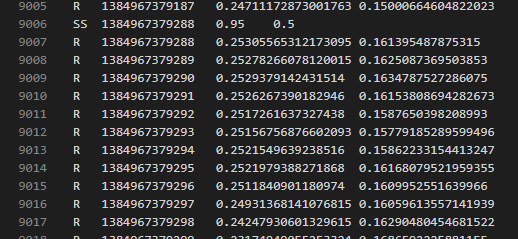
\includegraphics[width=0.8\linewidth]{resources/plikwejsciowy.png}
        \caption{Fragment pliku wejściowego}
        \label{fig:plikwejsciowy}
\end{figure}
Pierwsza kolumna reprezentuje typ odczytanych danych, zawiera ona dwie wartości: \textbf{SS} oraz \textbf{R}. SS oznacza zmianę mierzonego punktu, a wszyskie elementy R oznaczają wykonany pomiar. Kolejna kolumna przechowuje czas wykonania pomiaru w formacie \emph{UNIX} obliczanym w milisekundach. Jak można zauważyć, pomiar wykonywany jest z częstotliwością 1 ms, przez co odczytane wyniki powinny być dokładne. Trzeci oraz ostatni parametr to nieskalibrowane współrzędne punktów wejściowych, odpowiednio X i Y. Kalibrację danych opisano w sekcji \ref{ssec:calibration}.\par
Podobny format danych można znaleźć w bazie danych, zgodnie z podrozdziałem \ref{sec:shortdesc}, wraz z ich formatem.
\subsection{Format danych wyjściowych}
\label{ssec:exitdata}
Ten podrozdział opisuje format danych wyjściowych oraz pliki w jakich one są zapisywane.\par
Rezultatem działania programu jest trójka plików, plik \emph{.csv} zawierający obliczone dane, plik \emph{.png} będący reprezentacją graficzną obliczonych fiksacji oraz plik \emph{.log} przechowujący zrzut wykorzystania pamięci w czasie trwania aplikacji. Zapis danych odbywa się w momencie zakończenia obliczeń. Opis pliku graficznego został zaprezentowany w sekcji \ref{ssec:fixations}.\\
Plik \emph{.csv} zostaje zapisany w folderze \textbf{/result}, posiadając w nazwie tytuł pliku wejściowego, dołączając do niego datę wykonania programu, np. 1\_01\_1311201811.cal23\-10\-2019\-173857.csv.
Plik ten został zbudowany w sposób zaprezentowany na rysunku \ref{fig:exportfile}. Posiada on 6 parametrów, każdy odpowiadający pewnej obliczonej statystyce, bądź pomiarze zmierzonym w trakcie działania programu. Są to w kolejności od lewej do prawej:
\begin{figure}[H]
        \centering
        \captionsetup{justification=centering,margin=2cm}
        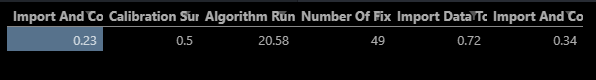
\includegraphics[width=0.8\linewidth]{resources/exportfile.png}
        \caption{Plik wyjściowy}
        \label{fig:exportfile}
\end{figure}
\begin{enumerate}[itemsep=1pt] 
        \item ImportAndConvertFileStatistic
        \item CalibrationSummaryTime
        \item AlgorithmRunTimeStatistic
        \item NumberOfFixationsCount
        \item ImportDataToDatabase
        \item ImportAndConvertDatabaseStatistic
\end{enumerate}
Wszystkie obliczone czasy podano w sekundach z dokładnością do 4 miejsc po przecinku. Pierwsza kolumna prezentuje czas trwania importu danych do pamięci oraz czas trwania konwersji plików do formatu czytelnego dla aplikacji, zgodnie z fragmentem \ref{ssec:importdata}. Następna kolumna przedstawia łączny czas trwania kalibracji współrzędnych wejściowych do formy układu współrzędnych odpowiadającej mierzonym punktom 'SS'. Trzecia kolumna prezentuje czas trwania algorytmu wykrywania fiksacji, a czwarta ilość odnalezionych fiksacji. Piąta i szósta kolumna mogą być puste, gdyż wykazują czas trwania importu danych do bazy danych, oraz odpowiednik importu i konwersji z pierwszej kolumny dla bazy danych dla dalszej analizy.\\
Celem obliczenia zużycia pamięci przez algorytm tworzony jest kolejny plik, tym razem z profilem pamięciowym aplikacji, czyli wykorzystaniem pamięci przez każdą linię utworzonego kodu. Fragment takiego pliku wynikowego zaprezentowano na rysunku \ref{fig:memoryfile}.
\begin{figure}[H]
        \centering
        \captionsetup{justification=centering,margin=2cm}
        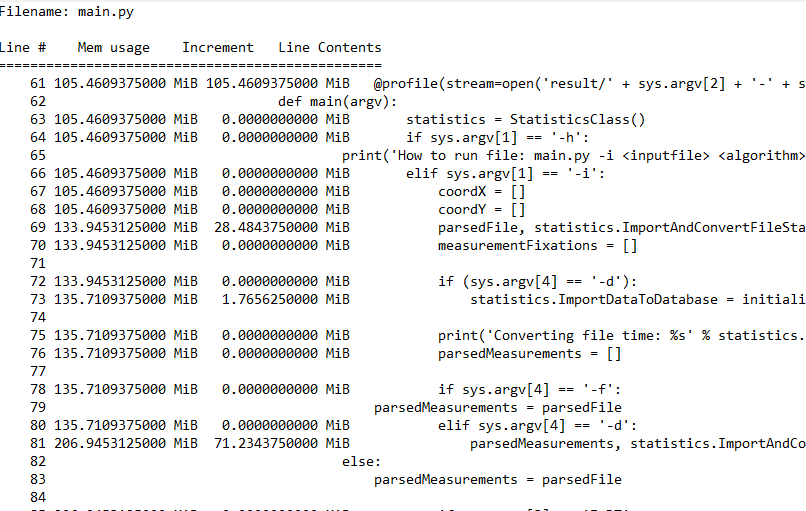
\includegraphics[width=\linewidth]{resources/memory_file.png}
        \caption{Fragment pliku ze zrzutem pamięci}
        \label{fig:memoryfile}
\end{figure}
Pierwsza kolumna prezentuje linię w pliku, druga wykorzystanie pamięci, trzecia różnicę w pomiarach pomiędzy poprzednią linią a obecną a ostatnia treść linii. Czwarta kolumna pozwala w łatwy sposób zinterpretować, jak dużo pamięci pobiera algorytm obliczania fiksacji.
\subsection{Prezentacja fiksacji}
\label{ssec:fixations}
\begin{figure}[H]
        \centering
        \captionsetup{justification=centering,margin=2cm}
        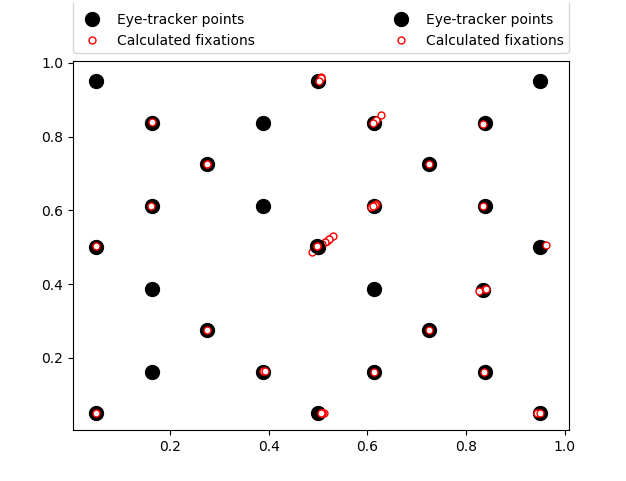
\includegraphics[width=0.8\linewidth]{resources/calculated_fixations.png}
        \caption{Przykład zaprezentowanych fiksacji}
        \label{fig:presentationfixation}
\end{figure}
Rysunek \ref{fig:presentationfixation} pokazuje sposób wyświetlania danych po wykonaniu konkretnego algorytmu. Czarne punkty przedstawiają punkty zaprezentowane użytkownikowi w trakcie przeprowadzenia badań, czyli punkty 'SS', a czerwone punkty prezentują wszystkie wykryte fiksacje. W celu zaprezentowania wszystkich elementów wykorzystano moduł matplotlib języka Python, który umożliwia takie rozwiązanie. Zezwala on również na przybliżanie otrzymanego wykresu, co pozwala na dokładniejszą analizę danych. Przykład ten zaprezentowano na rysunku \ref{fig:zoomedfixation}.
\begin{figure}[H]
        \centering
        \captionsetup{justification=centering,margin=2cm}
        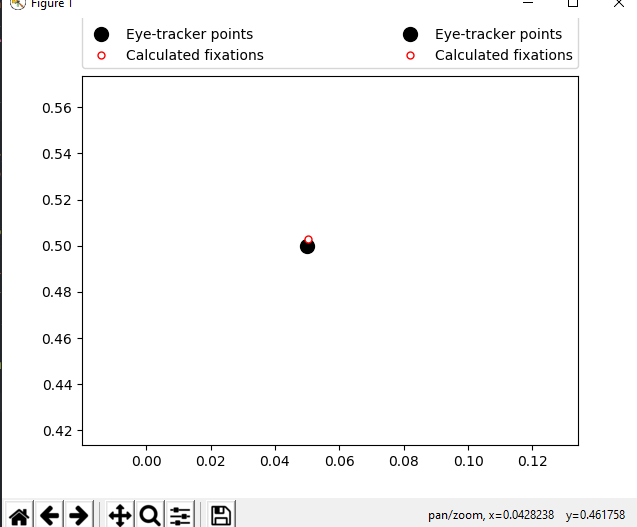
\includegraphics[width=0.8\linewidth]{resources/zoomed_fixation.png}
        \caption{Przybliżony podgląd fiksacji}
        \label{fig:zoomedfixation}
\end{figure}
W trakcie analizy danych, zaobserwowano iż w danych wejściowych istnieją dwa punkty 'SS' o wartościach $(0.5,0.5)$ co powoduje zwiększenie ilości mierzonych fiksacji w okolicach tego punktu, jak również brak pomiaru dla wartości $(0.3875,0.3875)$. Można to zaobserować na rysunku \ref{fig:presentationfixation}.
\section{Specyfikacja wewnętrzna aplikacji}
\label{sec:internal}
W tym podrozdziale przedstawiono informacje dotyczące sposobu implementacji algorytmów opisanych w rozdziale \ref{ssec:algorithms}. Przed tym, przedstawiono moduły języka Python wymagane do uruchomienia aplikacji, sposób ich wykorzystania, jak również opisano metodykę konwersji danych wejściowych na format czytelny dla algorytmów. Zaprezentowano także sposób połączenia z bazą danych MongoDB. Celem zwięzłości pokazanych fragmentów kodu, pominięto wyświetlanie inicjalizacji tablic, list oraz elementów nieistotnych dla działania algorytmów, typu pomiar czasu i pamięci. Ostatnie sekcje prezentują kod odpowiedzialny za pomiar czasu, profil pamięciowy oraz wyświetlanie danych.
\subsection{Wymagania aplikacji}
\label{ssec:apprequirements}
Żeby uruchomić skrypt \emph{run.ps1} opisany w sekcji \ref{ssec:parameters} na platformie Windows, należy ustawić parametr \emph{\textbf{ExecutionPolicy}} na wartość \emph{\textbf{Unrestricted}}. Można to wykonać za pomocą polecenia \emph{\textbf{Set-ExecutionPolicy Unrestricted}} w oknie konsoli PowerShell.\par
Zgodnie z fragmentem \ref{sec:tools}, aplikacja korzysta z języka \emph{Python}. Celem uruchomienia programu należy dodać do zmiennych środowiskowych ścieżki do środowiska Python. Przykład takich elementów pokazano na rysunku \ref{fig:path}.
\begin{figure}[H]
        \centering
        \captionsetup{justification=centering,margin=2cm}
        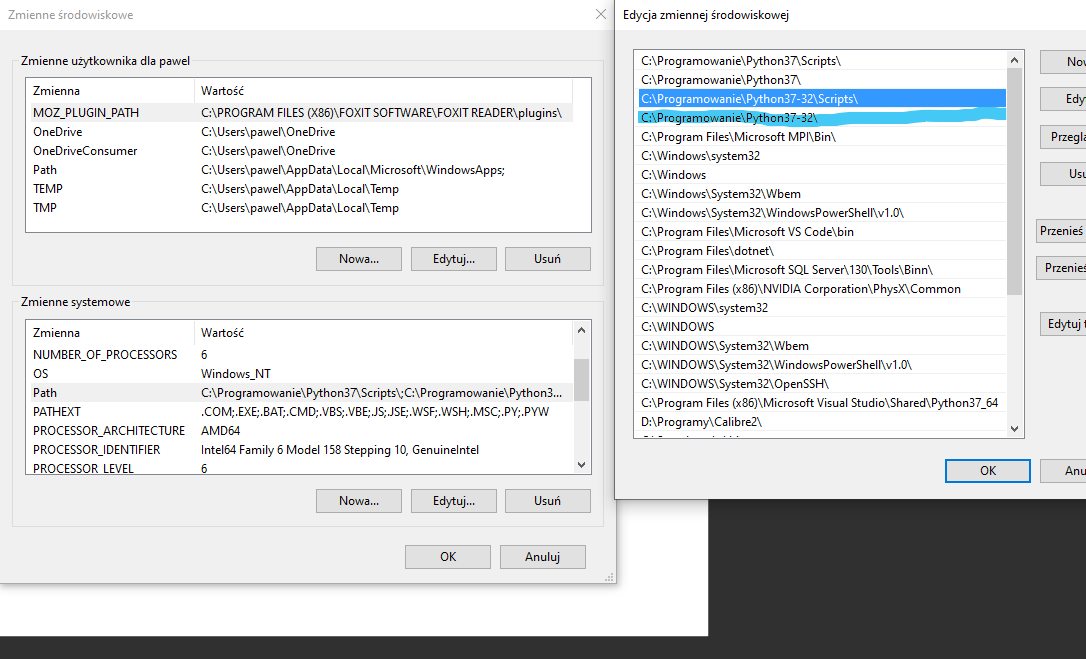
\includegraphics[width=\linewidth]{resources/path.png}
        \caption{Konfiguracja zmiennych środowiskowych}
        \label{fig:path}
\end{figure}
Projekt wymaga zainstalowania poniższych modułów języka Python, celem poprawnego działania konkretnych elementów aplikacji. Poniżej zaprezentowano te moduły, wraz z ich przeznaczeniem.\par
Wszystkie moduły można pobrać za pomocą pakietu \textbf{pip}, domyślnie instalowanego wraz z każdą instancją Pythona. Pierwszym modułem jest \textbf{NumPy}, które jest wiodącym pakietem przeznaczonym do bardziej skomplikowanych operacji na danych naukowych. W projekcie znalazł on zastosowanie m.in. w kalibracji danych wejściowych oraz przy danych dla modelu uczenia maszynowego. Pierwsze rozwiązanie przedstawiono w sekcj \ref{ssec:calibration}, gdzie wykorzystano metodę najmniejszych kwadratów celem obliczenia regresji liniowej punktów. Kolejną biblioteką jest \textbf{Matplotlib.pyplot}, umożliwiająca wyświetlanie danych wyjściowych. Moduł zaprezentowano w podrozdziale \ref{ssec:datashow}. Celem połączenia z bazą danych oraz prawidłową konwersją danych z tej bazy należało zainstalować moduły \textbf{pymongo} oraz \textbf{bson}. Zaprezentowano ich wykorzystanie w podsekcji \ref{ssec:db}. Kolejną ważną funkcjonalnością jest moduł \textbf{memory\_profiler}, któego celem jest wykonywanie zrzutu pamięciowego funkcji w ciągu działania aplikacji. Ostatnim modułem, który wykorzystuje się w sekcji \ref{ssec:machinelearningalg} jest podmoduł dla \textbf{NumPy}, mianowicie \textbf{scikit-learn}. Zawiera on wszystkie potrzebne narzędzia do tworzenia modeli oraz wykonywania przewidywań za pomocą uczenia maszynowego.\par
Domyślnie zainstalowanymi pakietami, które również znalazły swoje zastosowanie w pracy są pakiety \textbf{time}, \textbf{os}, \textbf{sys}. Odpowiadają one za pomiar czasu, obsługę plików oraz komunikację z systemem.\par
Ostatnim wymaganym elementem jest posiadanie bazy \textbf{MongoDB}. W tym celu należy zainstalować wybraną wersję pakietu ze strony \url{https://www.mongodb.com/}. Podczas instalacji automatycznie tworzona jest sesja pod wybranym przez użytkownika portem. Domyślną wartością jest \textbf{27017}. Metoda połączenia z bazą danych dla tego projektu pokazana jest w kodzie \ref{lst:connectDB}.
\subsection{Kalibracja danych wejściowych}
\label{ssec:calibrationtheory}
Ta sekcja ma za zadanie prezentację metodyki kalibracji danych wejściowych, jak również opis teoretyczny wykorzystanego zastosowania. Kod algorytmu znajduje się na listingu \ref{lst:calibration}.\par
Kalibracja danych ma za zadanie konwersję danych z czujnika ruchu do formatu danych na liniowym układzie współrzędnych odpowiadającym punktom. Jak można zauważyć na rysunku \ref{fig:plikwejsciowy}, współrzędne X i Y, dla danych typu \emph{'R'} w pliku wejściowym posiadają nietypowe wartości, co powoduje błędne działanie algorytmów wykrywania fiksacji. Rozwiązaniem problemu kalibracji jest zastosowanie metody najmniejszych kwadratów.\par
Zadaniem liniowej metody najmniejszych kwadratów jest znalezienie współczynników funkcji liniowej, przez którą przebiegają wszystkie punkty. W tej metodzie zakładamy iż nasze równanie wynosi $Ax = b$. Każda akcja wykonywana jest dwa razy, dla punktów osi X oraz Y.\par
Funkcja jest wywoływana osobno dla każdego punktu, ze względu na wstępną kalibrację przeprowadzoną przez urządzenie pomiarowe.
\begin{lstlisting}[language=Python, caption=Algorytm kalibracji, label={lst:calibration}]
import numpy as np
def calibrate(xList, yList):
        i = 1
        ...
        while i < len(xList):
                X.append([xList[i]**2,xList[i],yList[i]**2,yList[i]])
                Y.append([yList[i]**2,yList[i],xList[i]**2,xList[i]])
                ssxArr.append(xList[0])
                ssyArr.append(yList[0])
                i+=1
        
        x = np.linalg.lstsq(X,ssxArr,rcond=None)
        y = np.linalg.lstsq(Y,ssyArr,rcond=None)

        i = 1
        ...
        while i < len(xList):
                retX.append(x[0][0]*xList[i]**2 + x[0][1]*xList[i] + x[0][2]*yList[i]**2 + x[0][3]*yList[i])
                retY.append(y[0][0]*yList[i]**2 + y[0][1]*yList[i] + y[0][2]*xList[i]**2 + y[0][3]*xList[i])
                i += 1
        return retX, retY
\end{lstlisting}
W pierwszym kroku należy przygotować dane do dalszych obliczeń, co przedstawiono w liniach od 4 do 9. Tablice \textbf{ssxArr} oraz \textbf{ssyArr} są tablicami jednowymiarowymi o długości ilości pomiarów. Zawierają one wartość punktu 'SS', który jest skalibrowaną poprawną wartością. Dla równania liniowego jest on wektorem $b$. Tablice dwuwymiarowe \textbf{X} oraz \textbf{Y} odpowiadają macierzom współczynników $A$. Po umieszczeniu wszystkich elementów następuje obliczenie wartości $x$ za pomocą dostępnej metody \emph{np.linalg.lstsq}. Jako parametry przyjmuje ona wartości (A, b). Trzecim, opcjonalnym parametrem jest parametr odcięcia miejsc po przecinku dla małych wartości w macierzy $A$. Zauważono, iż dla dostępnych danych należy ustawić go na \emph{None}, żeby uzyskać dokładniejsze rezultaty.\par
Ostatnim krokiem algorytmu jest zapisanie obliczonych wartości punktów x oraz y. Następuje to za pomocą przyrównania ich do wartości z macierzy współczynników oraz zsumowania obliczonych wartości. Rezultatem algorytmu są skalibrowane punkty X oraz Y.
\subsection{Obsługa bazy danych}
W tym podrozdziale pokazano metody odpowiadające za obsługę bazy danych, w tym połączenie z nią oraz umieszczenie i wyciąganie danych.
\label{ssec:db}
\subsubsection{Połączenie z bazą danych}
\begin{lstlisting}[language=Python, caption=Połączenie z bazą danych, label={lst:connectDB}]
        import pymongo
        ...
        LOCALHOST = "mongodb://localhost:27017/"
        ...
        myclient = pymongo.MongoClient(LOCALHOST)
        mydb = myclient["mydatabase"]
\end{lstlisting}
Jak zaobserwowano w kodzie \ref{lst:connectDB} pakiet \textbf{PyMongo} umożliwia w bardzo prosty sposób połączenie z bazą danych. Trzecia linia kodu przedstawia zmienną przechowującą ścieżkę połączenia z bazą danych, a ostatnie dwie odpowiadają za połączenie oraz inicjalizację lub wybór instancji bazy danych. Te linie są wykorzystywane we fragmentach \ref{lst:insertDB} oraz \ref{lst:getFromDB} celem inicjalizacji zmiennych lokalnych odpowiadających za komunikację.
\subsubsection{Umieszczenie danych w bazie danych}
\label{ssec:insertDB}
Fragment dotyczący umieszczenia danych w bazie danych został zaprezentowany w kodzie \ref{lst:insertDB}. 
\begin{lstlisting}[language=Python, caption=Umieszczenie danych w bazie danych, label={lst:insertDB}]
def initialize_db(pointsList):
    ...
    myclient.drop_database("mydatabase")
    col = mydb["elements"]
    for element in list(pointsList):
            for value in element:
                    doc = collections.OrderedDict()
                    doc['Type'] = value.Type
                    doc['CoordX'] = value.CoordX
                    doc['CoordY'] = value.CoordY
                    doc['TimeStamp'] = value.TimeStamp
                    odbcarr.append(doc)
    col.insert_many(odbcarr)
    ...
\end{lstlisting}
Parametrem wejściowym funkcji jest lista wszystkich istniejących punktów. Fragment kodu w liniach 3 oraz 4 przedstawia inicjalizację elementów w bazie danych. W pierwszym kroku następuje wyczyszczenie istniejących elementów wraz z usunięciem instancji bazy danych, a potem utworzenie bazy danych \emph{"mydatabase"} z tabelą \emph{"elements"}. Jest to wykonywane za każdym razem, celem usunięcia poprzednich danych. Linie kodu od 6 do 12 przedstawiają umieszczenie elementów typu \textbf{OrderedDict} w tablicy. Tego typu obiekty zgodnie z dokumentacją, są najprostszym sposobem realizacji operacji INSERT w bazie danych dla większej ilości elementów. W linii 13 następuje umieszczenie elementów w tabeli.
\subsubsection{Wydobycie danych z bazy danych}
\label{ssec:getDB}
\begin{lstlisting}[language=Python, caption=Wydobycie danych z bazy danych, label={lst:getFromDB}]
def getFromDatabase():
    ...
    elements = mydb["elements"].find()
    for element in elements:
            item = Data(element['Type'], element['TimeStamp'], element['CoordX'], element['CoordY'])
            dataArray.append(item)
    i = 0
    loopFlag = True
    while loopFlag:
            for element in dataArray:
                    if i + 1 == len(dataArray):
                            retList.append(dataArray[i])
                            loopFlag = False
                            break
                    if dataArray[i + 1].Type == 'SS':
                            retList.append(dataArray[i])
                            break
                    retList.append(dataArray[i])
                    i += 1
            i += 1
            returnList.append(retList)
            retList = []
    ...
    \end{lstlisting}
Listing kodu \ref{lst:getFromDB} przedstawia rozwiązanie problemu wydobycia danych z tabeli w bazie danych. Linia 3 wykorzystując bibliotekę \textbf{MongoDB} pobiera wszystkie elementy za pomocą funkcji \emph{find()}. Można ją przyrównać do wykonania zapytania 
\begin{verbatim}
        SELECT * FROM mydatabase.elements;
\end{verbatim}
Następnym krokiem funkcji jest przetworzenie danych na dane czytelne dla algorytmów wykrywania fiksacji, implementację przedstawiono w liniach 4-6. Linie 9-22 odpowiadają za podział wszystkich punktów w celu umieszczenia ich w pamięci aplikacji do tablicy jednowymiarowej, której elementami są punkty przedzielone wartościami 'SS'.
\subsection{Przygotowanie danych do analizy}
\label{ssec:Dataanalysis}
\begin{lstlisting}[language=Python, caption=Przygotowanie danych do dalszej analizy, label={lst:datapreparation}]
        if sys.argv[3] == 'I-DT':
        print('Starting measurement using I-DT algorithm')
        for measurement in parsedMeasurements:
            print('Starting calibration')
            m1, convertingTime = convertPointsToCalibration(measurement)
            print('Ended calibration')
            coordX, coordY, timealgorithm, fixationsForPoint = calculateIdtAlgorithm(m1)
        print('Ending measurement using I-DT algorithm')
\end{lstlisting}
Na listingu \ref{lst:datapreparation} zaprezentowano metodykę przygotowania danych do analizy za pomocą algorytmów. Przykład przygotowuje dane dla algorytmu I-DT. Pierwsza linia przedstawia fragment pętli wybierającej odpowiedni algorytm, zgodnie z parametrami uruchomieniowymi zaprezentowanymi w sekcji \ref{ssec:parameters}. W pętli \textbf{for} elementem iterowanym jest lista odczytanych pomiarów. Każda z tych list jest oddzielona punktem 'SS'. W pierwszym kroku wykonywana jest kalibracja danych. Zwracanymi wartościami są lista punktów skalibrowanych - \emph{m1} oraz czas trwania konwersji. Kolejnym krokiem jest wykonanie algorytmu wykrywania fiksacji.
\subsection{Algorytm I-VT}
\label{ssec:implementivt}
\begin{lstlisting}[language=Python, caption=Kod algorytmu I-VT, label={lst:ivt}]
def calculateIvtAlgorithm(pointList):
    i = 0
    for element in pointList:
        velocity = 0
        if pointList[i].Type == 'SS':
            i += 1
            continue
        if i + 1 == len(pointList) - 1:
            velocity = math.sqrt(math.pow(pointList[i + 1].CoordX - pointList[i].CoordX, 2) + math.pow(pointList[i + 1].CoordY - pointList[i].CoordY, 2))
            if velocity < constants.FIXATION_VELOCITY_THRESHOLD:
                fixations.append(pointList[i])
                fixations.append(pointList[i + 1])
            break
        velocity = math.sqrt(math.pow(pointList[i + 1].CoordX - pointList[i].CoordX, 2) + math.pow(pointList[i + 1].CoordY - pointList[i].CoordY, 2))
        if (velocity < constants.FIXATION_VELOCITY_THRESHOLD):
            fixations.append(pointList[i])
        i += 1
    
    i = 0
    while i < len(fixations) - 1:
        velocity = math.sqrt(math.pow(fixations[i + 1].CoordX - fixations[i].CoordX, 2) + math.pow(fixations[i + 1].CoordY - fixations[i].CoordY, 2))
        if velocity < constants.FIXATION_VELOCITY_THRESHOLD:
            combineFixationsArray.append(fixations[i])
        else:
            if len(combineFixationsArray) != 0:
                coordX.append(sum(sumX.CoordX for sumX in combineFixationsArray) / len(combineFixationsArray))
                coordY.append(sum(sumY.CoordY for sumY in combineFixationsArray) / len(combineFixationsArray))
        i += 1
    return coordX, coordY, end - start, len(coordX)
\end{lstlisting}
W kodzie \ref{lst:ivt} przedstawiono implementację algorytmu I-VT w języku Python, zgodnie z pseudokodem \ref{lst:ivtpseudocode}. Jako parametr wejściowy funkcja otrzymuje podzieloną listę punktów zgodnie z opisem w sekcji \ref{ssec:Dataanalysis}. Główna pętla \textbf{for} iteruje po każdym punkcie z listy wejściowej. Zadaniem linii 5-7 jest pominięcie każdego punktu 'SS', gdyż nie jest on potrzebny do dalszych obliczeń. Wiersz 8 prezentuje warunek, gdy badany jest przedostatni i ostatni punkt z listy. Obliczana jest prędkość pomiędzy tymi punktami, i jeżeli warunek nr 2 zaprezentowany w pseudokodzie \ref{lst:ivtpseudocode} jest spełniony, dodaje się te punkty do listy fiksacji. Linie 14 do 17 prezentują działanie algorytmu dla punktów innych niż przedostatni i ostatni. Prędkość pomiędzy tymi elementami jest obliczana zgodnie ze wzorem:
\[
        \sqrt{(p[i+1].X - p[i].X)^2 + (p[i+1].Y - p[i].Y)^2}
\]
gdzie \emph{p} jest tablicą elementów, \emph{X} i \emph{Y} są współrzędnymi punktu a \emph{i} jest iteratorem tablicy.\\
Wiersze 20-28 odpowiadają za podział elementów na grupy fiksacji, zgodnie z linią 3 pseudokodu. Ten podział odbywa się za pomocą weryfikacji prędkości międzypunktowych. W wypadku znalezienia końca grupy fiksacji, następuje wydzielenie środka grupy fiksacji za pomocą równania:
\[
        \frac{\sum_{i = 0}^{n}{P_i}}{n}
\]
W tym równaniu P jest punktem X lub punktem Y, a N to liczba elementów w tablicy \emph{combineFixationsArray}.\\
Po przeanalizowaniu wszystkich punktów wejściowych, zwracane są następujące elementy: współrzędne X fiksacji, współrzędne Y fiksacji, czas trwania algorytmu oraz ilość fiksacji. Jak można zauważyć, w kodzie algorytmu znalazł się parametr \textbf{constants.FIXATION\_ VELOCITY\_ THRESHOLD}. Odpowiada on za próg prędkości opisany we fragmencie \ref{ssec:ivt}.
\subsection{Algorytm I-DT}
\label{ssec:implementidt}
W kodzie \ref{lst:idt} przedstawiono zaimplementowany algorytm I-DT, według pseudokodu opisanego w sekcji \ref{lst:idtpseudocode}. Jako parametr wejściowy ta funkcja przyjmuje podzieloną listę punktów. Ten podział zaprezentowano w sekcji \ref{ssec:Dataanalysis}. W 4 linii znajduje się główna pętla \textbf{while} algorytmu, działająca dopóki nie zostaną zanalizowane wszystkie punkty. Tak jak w algorytmie I-VT \ref{lst:ivt}, punkty 'SS' są pomijane, co zapisano w liniach 5-7. Następnie należy przygotować wstępne okno do przeprowadzenia obliczeń. Zgodnie z dokumentacją, potrzeba do tego celu parametru czasowego rozmiaru okna, który określono jako \textbf{constants.WINDOW\_TIME\_THRESHOLD}. Tworzenie okna pokazano w pętli \textbf{while} pomiędzy liniami 8-14. Dwie zmienne lokalne \textbf{timeStart} i \textbf{currTime} służą do pomiaru czasu. W wypadku przekroczenia ilości elementów w liście wejściowej pętla główna jest przerywana. Po dodaniu wszystkich elementów zgodnych z warunkiem pętli należy obliczyć dyspersję w oknie. Zastosowano do tego następujący wzór:
\[
        D = (\max{P_X} - \min{P_X}) + (\max{P_Y} - \min{P_Y})
\]
Kolejnym krokiem, po przygotowaniu wstępnego okna, jest porównanie czy dyspersja spełnia warunek graniczny opisany w kroku 3 pseudokodu. Warunek graniczny przechowywany jest w zmiennej \textbf{constants. DISPERSION\_THRESHOLD}. W wypadku gdy dyspersja jest mniejsza, należy dodawać kolejne punkty aż zostanie przekroczony warunek graniczny, co zaprezentowano w pętli \textbf{while} pomiędzy wierszami 22 i 27. Po przekroczeniu wartości granicznej zostaje dodany do tablic wyjściowych punkt centralny okna, obliczony za pomocą wzoru
\[
        P = \sum_{i = 0}^{n}{P_i}
\]
P może być punktem X lub Y. Po tym okno jest czyszczone do momentu spełnienia warunku granicznego, i algorytm jest wykonywany do skończenia punktów.\\
Algorytm zwraca listę współrzędnych X i Y, czas trwania algorytmu oraz ilość fiksacji.
\begin{lstlisting}[language=Python, caption=Kod algorytmu I-DT, label={lst:idt}]
def calculateIdtAlgorithm(pointsList):
        timeStart = int(pointsList[0].TimeStamp)
        countPoints = len(pointsList)
        while i < countPoints - 1:
                if pointsList[i].Type == 'SS':
                        i += 1
                        continue
                currTime = int(pointsList[i].TimeStamp)
                while currTime - timeStart <= constants.WINDOW_TIME_THRESHOLD:
                        windowList.append(pointsList[i])
                        i += 1
                        if i >= countPoints:
                                break
                        currTime = int(pointsList[i].TimeStamp)
                if i >= countPoints:
                        break
                if len(windowList) > 1:
                        Dispersion = (max(maxX.CoordX for maxX in windowList) - min(minX.CoordX for minX in windowList)) + (max(maxY.CoordY for maxY in windowList) - min(minY.CoordY for minY in windowList))
                while len(windowList) > 1:
                        if Dispersion <= constants.DISPERSION_THRESHOLD and len(windowList) > 1:
                                while (Dispersion < constants.DISPERSION_THRESHOLD):
                                        windowList.append(pointsList[i])
                                        i += 1
                                        if i >= countPoints:
                                                break
                                        Dispersion = (max(maxX.CoordX for maxX in windowList) - min(minX.CoordX for minX in windowList)) + (max(maxY.CoordY for maxY in windowList) - min(minY.CoordY for minY in windowList))
                                if i >= countPoints:
                                        break
                                coordXList.append(sum(sumX.CoordX for sumX in windowList) / len(windowList))
                                coordYList.append(sum(sumY.CoordY for sumY in windowList) / len(windowList))
                        else:
                                windowList.pop(0)
                if i <= countPoints - 1:
                        timeStart = int(pointsList[i].TimeStamp)
        return coordXList, coordYList, end - start, len(coordXList)
\end{lstlisting}
\subsection{Algorytm wykorzystujący uczenie maszynowe}
\label{ssec:machinelearningalg}
Opis teoretyczny biblioteki przeznaczonej do wykorzystywania uczenia maszynowego bazuje na pracy \cite{MLPython}.\par 
Jak opisano w rozdziale \ref{ssec:machinelearning}, uczenie maszynowe ze względu na rozwój technologiczny stało się jedną z najczęściej wykorzystywanych technologii, szczególnie przy analizie danych. W celu użycia tych rozwiązań, w języku Python należy wykorzystać pakiet \textbf{scikit-learn}. Zezwala on na stworzenie projektu z wykorzystaniem wielu dostępnych klasyfikatorów uczenia maszynowego np. k-NN\footnote{k najbliższych sąsiadów}, SVC, regresji liniowej.\\
Celem wykonywania przewidywań w aplikacji wykorzystano model regresji logistycznej. Jest to metoda statystyczna, której zadaniem jest przewidywanie wyników dla klas binarnych, przez co znajduje ona idealne zastosowanie dla algorytmów wykrywania fiksacji. Różni się ona od regresji liniowej danymi wyjściowymi. Podczas gdy regresja liniowa jako wynik prezentuje dane ciągłe, to regresja logistyczna przyjmuje wartości stałe. Oznacza to, iż regresja liniowa może przewidywać więcej wartości. Wyróżnia się jednak dodatkowe typy regresji logistycznych, takie jak binarna regresja, gdzie wynikiem może być podział na to czy wiadomość należy do spamu czy nie oraz wielomianowa regresja, gdzie rezultatem może być przykładowo typ wina.\\
Celem uruchomienia algorytmu uczenia maszynowego należy zbudować model danych. Przykład takiego modelu zaprezenotwano w kodzie \ref{lst:mlhelperclass}. Ten kod przedstawia konstruktor klasy pomocniczej \textbf{MLHelper}. Posiada ona cztery elementy: informacje o punkcie, obliczoną prędkość pomiędzy tym punktem oraz następnym, odległość międzypunktową oraz wartość fiksacji w tym punkcie obliczoną za pomocą algorytmu \ref{ssec:ivt}. Podczas projektowania aplikacji próbowano dodać dodatkowe parametry takie jak odległości w oknie dla punktu oraz dane statystyczne dotyczące okna, jednak powodowały one przesycenie modelu, co powodowało błędy w obliczeniach oraz brak fiksacji na wyjściu. Drugim powodem braku ich implementacji był bardzo duży przyrost czasu przeznaczanego na przygotowanie modelu danych, ze względu na dużą ilość danych, średnio kilkaset tysięcy na plik.
\begin{lstlisting}[language=Python, caption=Konstruktor klasy pomocniczej, label={lst:mlhelperclass}]
def __init__(self, Type, CoordX, CoordY, TimeStamp,  *args, **kwargs):
        self.Data = Data(Type, TimeStamp, CoordX, CoordY)
        self.VelocityBetweenPoints = float(0)
        self.DistancesBetweenPoints = float(0)
        self.IsFixation = bool
\end{lstlisting}
W kodzie \ref{lst:mlalgorithm} przedstawiony został algorytm wykorzystujący uczenie maszynowe. Początek algorytmu, czyli linie od 2 do 5 przedstawiają inicjalizację tablic typu \textbf{numpy.array}, które umożliwiają na bardziej skomplikowane operacje na tablicach, podobne do tych używanych w języku R oraz MatLAB. Przykładem wykorzystania takich operacji jest linia 14, gdzie zdecydowano na przekazanie tylko wartości 'VEL', 'DBP' oraz 'FIX' do modelu danych. Na początku funkcji inicjalizowane są tablice X1, Y1 dla danych treningowych, oraz X2, Y2 dla danych testowych. Następnie w liniach 6-15 przedstawiono pobranie danych z parametrów wejściowych funkcji oraz ich konwersję na format czytelny dla biblioteki \textbf{numpy}. Należało wykonać konwersję z obiektu \textbf{class} na słownik, gdyż obiekt \textbf{pd.DataFrame} przyjmuje listę obiektów iterowalnych jako swój parametr. Przykład realizacji takiej konwersji pokazano na listingu \ref{lst:iter}.
\begin{lstlisting}[language=Python, caption=Iterator, label={lst:iter}]
        def __iter__(self):
                yield 'Data', self.Data
                yield 'VEL', self.VelocityBetweenPoints
                yield 'DBP', self.DistancesBetweenPoints
                yield 'FIX', 1 if self.IsFixation == True else 0
\end{lstlisting}
W linii 18 postawiono warunek podziału ile obiektów ma służyć jako trening dla modelu, a ile przeznaczyć na testowanie. Zdecydowano się na podzielenie zbioru danych na zbiory: 10\% danych treningowych, 90\% danych testowych. Należało te dane połączyć, co przedstawia funkcja \textbf{np.concatenate[X,Y]}, przyjująca dwie tablice o tych samych wymiarach jako swoje parametry.\\
W linii 26 po wyborze typu modelu następuje jego uczenie za pomocą tablic testujących. Następny wiersz przedstawia wykonanie predykcji. Po obliczeniu wszystkich wartości wynikowych należy zbadać dokładność algorytmu, co zostało pokazane w linii 29. \textbf{Numpy} udostępnia funkcje sprawdzające dokładność oraz precyzję klasyfikatorów uczenia maszynowego.
\begin{lstlisting}[language=Python, caption=Algorytm wykorzystujący uczenie maszynowe, label={lst:mlalgorithm}]
def calculateML(pointList):
        start = time.process_time()
        XArr = np.empty([1,3])
        YArr = np.empty([1])
        XArr2 = np.empty([1,3])
        YArr2 = np.empty([1])
        for i, point in enumerate(pointList):
        tmpArr = list()
        for item in point:
                el = dict(item)
                tmpArr.append(el)
        values = pd.DataFrame(tmpArr, columns=['Data', 'VEL', 'DBP', 'FIX'])
        array = values.values
        X = array[:,0:3]
        Y = array[:,3]
        Y=Y.astype('int')
        if len(X) != len(Y):
                print('W punkcie ' + i + ' jest bład')
        if i < 3:
                XArr = np.concatenate([XArr,X])
                YArr = np.concatenate([YArr,Y])
        else:
                XArr2 = np.concatenate([XArr2,X])
                YArr2 = np.concatenate([YArr2,Y])
        print(XArr[1:,1:])
        model = LogisticRegression()
        model.fit(XArr[1:,1:], YArr[1:])

        prediction = model.predict(XArr2[1:,1:])

        ite = accuracy_score(YArr2[1:], prediction)
        print(ite)
        endXArr = np.concatenate([XArr[1:,:],XArr2[1:,:]])
        endYArr = np.concatenate([YArr[1:],prediction])
        endAll = np.c_[endXArr,endYArr]

        retX = []
        retY = []
        print(endAll)
        for item in endAll:
        if item[3] == 1:
                retX.append(item[0].CoordX)
                retY.append(item[0].CoordY)
        end = time.process_time()
        return retX, retY, len(retX), end - start, ite
\end{lstlisting}

\subsection{Prezentacja wyników}
\label{ssec:datashow}
\begin{lstlisting}[language=Python, caption=Wyświetlanie wyników, label={lst:plot}]
        import pyplot as plt
        ...
        plt.plot(m1[i].CoordX, m1[i].CoordY, 'ko', markersize=10, label='Eye-tracker points' if i == 0 else "")
                ...
                coordX, coordY, timealgorithm, fixationsForPoint = calculateIdtAlgorithm(m1)
                plt.plot(coordX, coordY, 'wo', markersize=5, markeredgecolor='r', label='Calculated fixations')
                ...
            plt.legend(bbox_to_anchor=(0., 1.02, 1., .102), loc=3, ncol=2, mode="expand", borderaxespad=0.)
            plt.show()
\end{lstlisting}
Listing \ref{lst:plot} prezentuje wykorzystanie biblioteki \textbf{pyplot} odpowiadającej za tworzenie wykresów oraz wyświetlanie punktów na układzie współrzędnych w języku Python. Funkcja \emph{plot()} przyjmuje jako parametry wejściowe następujące wartości: X, Y, sposób prezentacji, rozmiar linii/punktu, legendę. Celem wyświetlenia wartości należy użyć funkcji \textbf{plt.show()}. Otwiera ona nowe okno z naniesionymi wartościami. Przykład takiego okna zaprezentowano na rysunku \ref{fig:presentationfixation}.
\subsection{Pomiar czasu}
\label{ssec:timemethod}
W trakcie wykonywania aplikacji wykonywany jest pomiar czasu działania różnych funkcji aplikacji. W tym celu została wykorzystana biblioteka \textbf{time}. W kodzie \ref{lst:time} zaprezentowano sposób działania biblioteki. Funkcja \textbf{time.process\_time} zwraca obecny czas systemowy w sekundach, więc różnica tych wartości prezentuje czas trwania danego kodu.
\begin{lstlisting}[language=Python, caption=Pomiar czasu, label={lst:time}]
    start = time.process_time()
        # wykonywana akcja
    end = time.process_time()
    return ..., end - start, ...
\end{lstlisting}
\subsection{Pomiar wykorzystania pamięci}
\label{ssec:memorymethod}
W celu przeprowadzenia pomiaru wykorzystania pamięci w aplikacji należy użyć biblioteki \textbf{memory\-profiler}. Sposób implementacji przedstawiono w kodzie \ref{lst:memory}. Ten moduł został użyty do całej aplikacji, przez zdefiniowanie go przed funkcją \textbf{main}. Ta biblioteka wypisuje zużycie pamięci w MB przez każdą linijkę aplikacji, oraz zapisuje ją do pliku poprzez użycie parametru 'stream'. W wypadku aplikacji zastosowano precyzję do 4 miejsc po przecinku, ze względu na zakładaną możliwość mniejszego zużycia pamięci przez podstawowe algorytmy. Określenie tej precyzji znajduje się w parametrze \emph{precision}.
\begin{lstlisting}[language=Python, caption=Pomiar wykorzystania pamięci, label={lst:memory}]
@profile(stream=open('result/' + sys.argv[2] + '-' + sys.argv[3] + '.log','w+'), precision=4)
def main(argv):
\end{lstlisting}
Na rysunku \ref{fig:memoryfile} zaprezentowano fragment zastosowania tej biblioteki.
